\documentclass[9pt]{beamer}
% ****************
% ***** INFO *****
% ****************
\usepackage[english]{babel}
\title[University of Calabria]{Study and data analysis of turbulence numerical models in mid-atmospheric boundary layer.}
\subtitle{Supervisors: Prof. Leonardo Primavera,\\ \quad \quad \quad \quad \quad \, \, Prof. Fabio Lepreti.}
\author[Name Surname]{ Francesco De Rose. \textbf{ID}: 256865}
\institute[]{University of Calabria, Physics department, Rende (CS)}
\newcommand{\currentyear}{\the\year} % \currentyear
\newcommand{\nextyear}{\the\numexpr\year+1\relax} % \nextyear
\date{\currentyear/\nextyear} % or \today
\setbeamertemplate{frametitle}[default][center]

% *******************
% ***** PROJECT *****
% *******************
\definecolor{main}{HTML}{0000FF}
\setbeamercolor{structure}{fg=main}

% *****************
% ***** THEME *****
% *****************
\usepackage{wrapfig}
\usetheme{Luebeck}
\usepackage{helvet}
\renewcommand{\familydefault}{\sfdefault}
\setbeamertemplate{frametitle continuation}{\gdef\beamer@frametitle{}}
\setbeamertemplate{footline}[frame number]

% *****************
% ***** CODE *****
% *****************
\newcommand\Fontvs{\fontsize{4}{6.0}\selectfont}
\newcommand\Fontvi{\fontsize{6}{7.2}\selectfont}
\newcommand\Fonttab{\fontsize{12}{7.2}\selectfont}
\usepackage{listings}
\lstdefinestyle{java}{
    backgroundcolor=\color{white},
    basicstyle=\ttfamily\scriptsize,
    breaklines=true,
    commentstyle=\color{gray},
    keywordstyle=\color{blue},
    stringstyle=\color{magenta},
    identifierstyle=\color{black},
    numberstyle=\color{gray},
    language=Java
}
\lstdefinestyle{cpp}{
    backgroundcolor=\color{white},
    basicstyle=\ttfamily\scriptsize,
    breaklines=true,
    commentstyle=\color{gray},
    keywordstyle=\color{blue},
    stringstyle=\color{magenta},
    identifierstyle=\color{black},
    numberstyle=\color{gray},
    language=C++
}
\lstdefinestyle{py}{
    backgroundcolor=\color{white},
    basicstyle=\ttfamily\scriptsize,
    breaklines=true,
    commentstyle=\color{gray},
    keywordstyle=\color{blue},
    stringstyle=\color{magenta},
    language=Python
}
\lstdefinestyle{js}{
    backgroundcolor=\color{white},
    basicstyle=\ttfamily\scriptsize,
    breaklines=true,
    commentstyle=\color{gray},
    keywordstyle=\color{blue},
    stringstyle=\color{magenta},
    identifierstyle=\color{black},
    numberstyle=\color{gray},
    language=JavaScript,
    escapechar=@
}
\lstdefinestyle{sh}{
    basicstyle=\ttfamily\scriptsize,
    breaklines=true,
    commentstyle=\color{gray},
    keywordstyle=\color{blue},
    stringstyle=\color{magenta},
    identifierstyle=\color{black},
    numberstyle=\color{gray},
    language=bash
}

% **********************
% ***** ALGORITHMS *****
% **********************
\usepackage{algorithm}
\usepackage{algpseudocode}

% *****************
% ***** UTILS *****
% *****************
\usepackage{xcolor}
\usepackage{graphicx}
\graphicspath{./figures/}
\usepackage{multimedia}
% ********************
% ***** DOCUMENT *****
% ********************
\begin{document}

% **********************
% ***** TITLEPAGE ******
% **********************
\begin{frame}{}
\vspace{\fill}


\begin{figure}[htbp] % htbp stand for "here", "top", "bottom", "page"

\includegraphics[scale=0.50]{/figures/logof.jpg} 
\end{figure}

\vspace{\fill}

\Large
\color{main}
\inserttitle

\medskip

\large
\color{black}
\insertsubtitle

\vspace{\fill}

\footnotesize
\insertinstitute

\vspace{\fill}

\textbf{Author:} \insertauthor

\medskip

\insertdate

\vspace{\fill}
\end{frame}

%\item \href{https://example.com/}{\underline{\color{main}{Link}}}
% *****************
% ***** START *****
%    \item \textbf{Bold}
%    \item \textit{Italic}
%    \item \texttt{Monospaced}
%    \item \underline{Underlined}
% *****************
\begin{frame}[allowframebreaks]{\textbf{Introduction}}
\Fonttab
\begin{itemize}

\item This presentation focuses on computation of the trends in the occurrence of atmospheric circulation patterns using a python script (.ipynb file).
\item In the case studied, a brief explanation of the state of the art of these methods will be explained.
\item All the computations and figures have been obtained using different python libraries (seaborn, xarray, scipy to name a few). \\The dataset (1.9GB size) used contains 500 hPa geopotential values recorded each day at 12:00UTC  from 01011980 to 11072025 relative to this area: 
$70^\circ N:35^\circ S; -20^\circ W:30^\circ E$ on an horizontal grid $0.25^\circ \times 0.25^\circ$.  
\end{itemize}
\begin{eqnarray}
\boxed{\Phi  = \int_{0}^{z}\, \mathbf{g}\, dz^{\prime} }
\end{eqnarray}
\end{frame}

\begin{frame}[allowframebreaks]{\textbf{ITFA and NWP models}}
\Fontvi
The effects that climate change driven turbulence has on aviation over Europe is a serious matter, namely:
\begin{enumerate}
\item Turbulence $\longrightarrow$ microscale phenomenon . A scale mismatch makes direct forecasting extremely challenging from a meteorological standpoint.
\item Turbulent eddies exist across a vast spectrum of sizes . Atmospheric turbulence ranges from 100s of km down to just cm, creating complexity in prediction models.
\item Aircraft bumpiness peaks at aircraft scale eddies . Commercial aircraft experience the most pronounced turbulence when encountering eddies $\sim$ 100 meters in size, roughly matching the aircraft dimensions $\longrightarrow$ No safe prediction for atmospheric motion at the 100 meter scale.
\item Energy cascades from larger to smaller scales . Most energy in aircraft-scale turbulent eddies originates from larger atmospheric motions that cascade downward, providing a pathway for indirect prediction.
\item Larger scales are observable and resolvable . Current weather observation networks and numerical weather prediction models can effectively capture and resolve these larger-scale atmospheric features.
\item Empirical forecasting methods bridge the scale gap . Practical "rules of thumb" can link observable large scale atmospheric patterns to aircraft-scale turbulence predictions.
\end{enumerate}
\end{frame}

\begin{frame}[allowframebreaks]{\textbf{Presentation objective}}
\Fonttab
The goal is to investigate the extent to which changes in atmospheric dynamics amplify the impacts of climate change on aviation turbulence at \colorbox{orange}{regional scales}.
\centering
\movie[externalviewer]{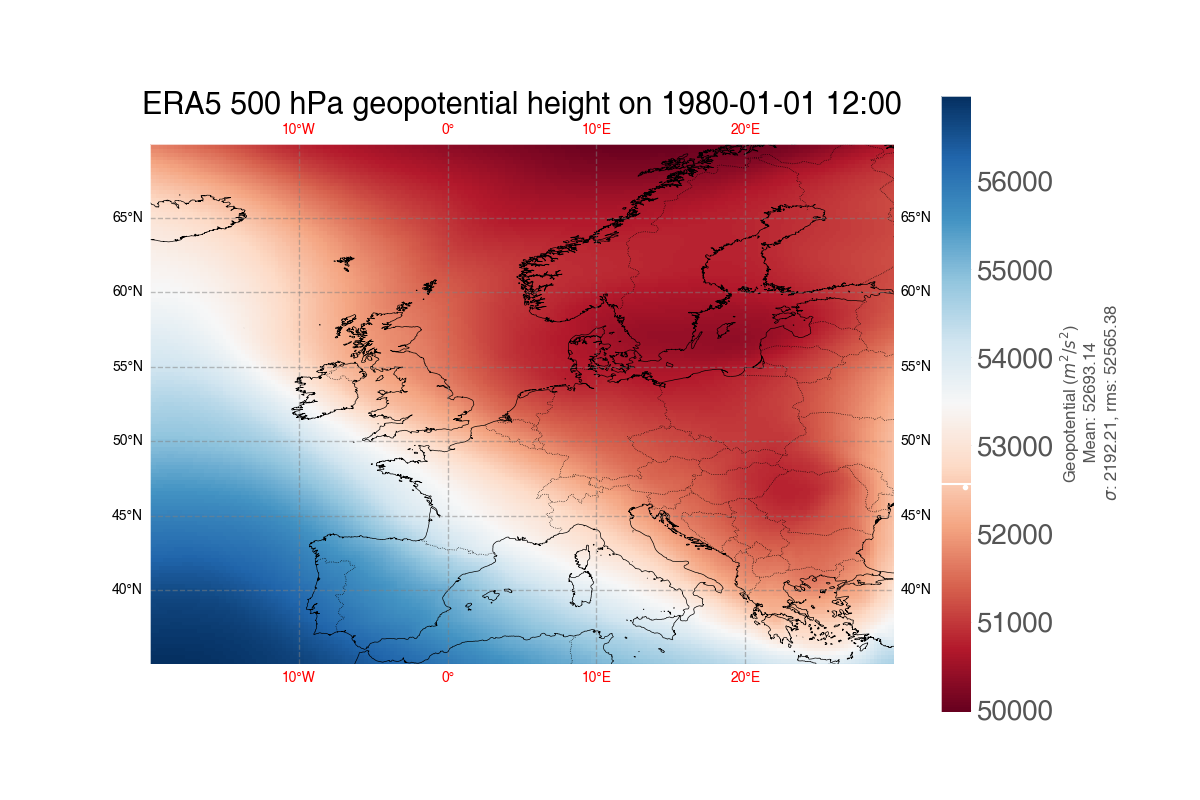
\includegraphics[width=0.5\textwidth]{figures/map_00.png}}{figures/video.mp4}\\
With long enough data (45 years) one can derive some spatial pattern of key
diagnostics (mainly Ellrod's indices TI1 not TI2 \cite{ellrod1992}) related to aviation turbulence episodes. The video shows along the colorbar the mean and RMS of the plev daily value.
\end{frame}

\begin{frame}[allowframebreaks]{\textbf{Components and algorithms}}
\Fonttab
This forecasting method integrates multiple turbulence diagnostics, each weighted based on observations. A set of turbulence indices are computed from \colorbox{orange}{ERA5 reanalysis dataset} \cite{faranda2024} at each grid point.  Upper-level algorithms:
 \begin{enumerate}[I]
\item Horizontal temperature gradient;
\item Turbulence Index 1 (TI1);
\text{Mid-level algorithms\cite{sharman2006}:}
\begin{enumerate}[I]
\item \colorbox{orange}{TI1}; 
\item Wind speed $\times$ horizontal deformation.
\item many others ...
\end{enumerate}
\end{enumerate}
\end{frame}

\begin{frame}[allowframebreaks]{\textbf{Clear Air Turbulence (CAT) significance}}
\Fontvi
\begin{center}
\begin{exampleblock}{Why it's important?}
CAT is defined as high-altitude aircraft bumpiness occurring away from significant cloudiness and thunderstorm activity.  Nonetheless, \textbf{CAT} accounts for half of all encounters with turbulence, despite occurring in seemingly benign atmospheric conditions.
\begin{enumerate}
    \item \textbf{Morphology of patterns} By focusing on the morphology of large-scale \colorbox{orange}{geopotential patterns}, that have become more frequent over the last four decades in ERA5 data , the most-encountered spatial patterns of key turbulence diagnostics can be identified.
    \item \textbf{Information lost} This resolution allows for the detection of temporal trends in dynamics (from hours to inter-annual decadal timescales) associated with spatial patterns, ensuring uniform spatial and temporal coverage.
\end{enumerate}
\Fontvi
\text{See for example \url{https://turbli.com/maps/world-turbulence-map/}.}
\end{exampleblock}
\end{center}
\end{frame}


\begin{frame}[allowframebreaks]{\textbf{Analog searching method and pseudo-code } \cite{alberti2024}}
\Fontvs
\begin{algorithmic}
\Procedure{FindAnalogs}{$maps, reference\_map, q\_quantile$}
    \Comment{Euclidean distances}
    \State $distances \gets \text{empty list}$
    \For{\textbf{each} $map\_i$ \textbf{in} $maps$}
        \State $distance \gets \text{EuclideanDistance}(map\_i, reference\_map)$
        \State $distances.\text{append}(distance)$
    \EndFor
    \Comment{Quantile determination}
    \State $threshold \gets \text{CalculateQuantile}(distances, q\_quantile)$
    \State $analogs \gets \text{empty list}$
    \For{\textbf{each} $map\_i$ \textbf{and} $distance\_i$ \textbf{in} $maps, distances$}
        \If{$distance\_i \le threshold$}
            \State $analogs.\text{append}(map\_i)$ \Comment{Store map or its date/identifier}
        \EndIf
    \EndFor
    \State \textbf{return} $analogs$
\EndProcedure
\Procedure{AnalyzeAnalogTrends}{$analog\_dates, time\_interval\_length$}
    \Comment{Trend Analysis}
    \State $sub\_intervals \gets \text{DivideTimeIntoSubintervals}(analog\_dates, time\_interval\_length)$
    \State $N\_t \gets \text{empty list}$ \Comment{List to store number of analogs per sub-interval}
    \For{\textbf{each} $sub\_interval$ \textbf{in} $sub\_intervals$}
        \State $count \gets \text{CountAnalogsInSubinterval}(sub\_interval, analog\_dates)$
        \State $N\_t.\text{append}(count)$
    \EndFor
    \State $a, b \gets \text{LinearBestFit}(time\_points, N\_t)$ \Comment{$N(t) = at + b$}
    \State \textbf{return} $a, b$
\EndProcedure
\Procedure{ReconstructCompositeMaps}{$analog\_dates, field\_of\_interest$}
    \Comment{Composite map reconstruction}
    \State $composite\_map \gets \text{empty map}$
    \State $total\_fields \gets 0$
    \For{\textbf{each} $date$ \textbf{in} $analog\_dates$}
        \State $field\_data \gets \text{RetrieveFieldData}(date, field\_of\_interest)$
        \State $composite\_map \gets composite\_map + field\_data$ \Comment{Sum or average fields}
        \State $total\_fields \gets total\_fields + 1$
    \EndFor
    \State $composite\_map \gets composite\_map / total\_fields$ \Comment{Average the composite map}
    \State \textbf{return} $composite\_map$
\EndProcedure
\end{algorithmic}
\end{frame}

\begin{frame}[allowframebreaks]{\textbf{Figures and discussions: what's been plotted}}
\Fonttab
\begin{enumerate}
\item \textbf{Annual trend} to compare the effects of climate change on plev, based on the dataset time and space indices.
\item \textbf{Maps at specific times} $\, \Phi(\mathbf{x},t) $ to show the overall behavior in the past 45 years.
\item \textbf{Contour plots} representing spatial coordinate along the horiz.plane, \underline{for a single hour of a day/month/year} and the plev $(\mathbf{x},t)$ as the plot intensity.
\item \textbf{Euclidian distances distribution and linear fits}\\ For suitable reference days, the \colorbox{orange}{linear fit} and \colorbox{orange}{confidence interval for a consistent trend} has been computed.
\item \textbf{TI1} For suitable time periods, the trend for the \colorbox{orange}{turbulence index} has been computed, namely the horizontal gradient of the converted geopotential.
\end{enumerate}
\end{frame}
% ******* TABLES *********
\begin{frame}[allowframebreaks]{\textbf{Tables}}
\Fontvi
\begin{table}
    \centering
    \begin{tabular}{|c|c|c|c|c|c|}
        \hline
        \textbf{Ref.day} & \textbf{Analog counts}&\textbf{a} & \textbf{95\% CI}
 & q & trend \\
        \hline 
        16619 & 1129228 & 17903.6  & 9140.8233, 26666.3767 & 0.98 & Yes\\
        \hline
    \end{tabular}
    \caption{Coefficients and parameters for runs in the set of 5th period of 9 years 20160702-20250702. The quantiles used have been \colorbox{orange}{0.98, 0.99, 0.995} as in \cite{alberti2024}. The dataset has been centered and standardized (each map before distance computation) to delete anomalies and \colorbox{orange}{seasonal variabilities} in analogs computation.}
    \label{tab:1}
\end{table}

\begin{table}
    \centering
    \begin{tabular}{|c|c|c|c|c|c|}
        \hline
        Period:&80'-89' &89'-98'  & 98'-07' & 07'-16' & 16'-25' \\
        \hline
       Analog count& 1059876& 1083430 &1124200   &1123762 & 1129228  \\
        \hline
    \end{tabular}
    \caption{Analog counts for all 5 periods 19800101-20250711. The quantiles used has been 0.98, as in \cite{alberti2024}; it has been chosen to highlight the \colorbox{orange}{2\% closest patterns}. For further information refer to the "h.press.analogue.ipynb" file and the "results.fit.txt" in the directory.}
    \label{tab:1}
\end{table}
\end{frame}
% ******* FIGURES ********
\begin{frame}[allowframebreaks]{\textbf{Annual trend}}
\centering
\movie[externalviewer]{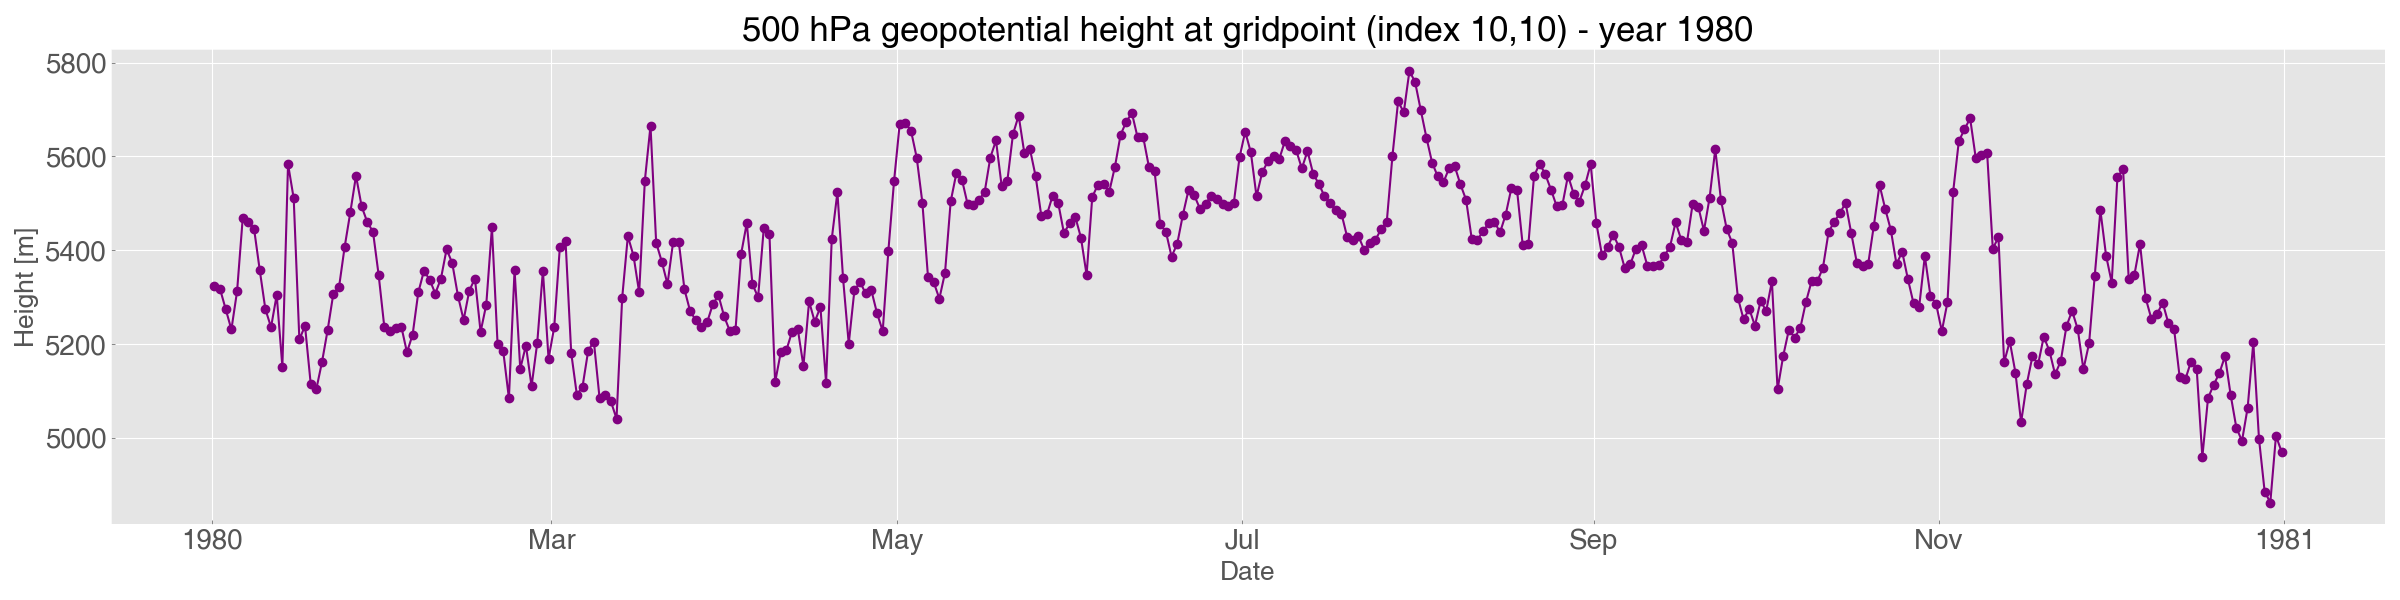
\includegraphics[width=0.95\textwidth]{figures/atrend/atrend_1980.png}}{figures/atrend/output.mp4}\\
\colorbox{orange}{Annual trend} video of the 500 hPa geopotential variable plev selected at a specific index of the spatial grid. Information on the dataset:
\begin{enumerate}
\item Dimensions:     time: 16628lon: 201lat: 141plev: 1
\item Coordinates:
    time     1980-01-01T12:00:00 ... 2025-07-11...
    lon   -20.0 -19.75 -19.5 ... 29.75 30.0
    lat    70.0 69.75 69.5 ... 35.5 35.25 35.0
    plev    5e+04
\item Attributes:
CDI :
    Climate Data Interface version 2.1.1 (\url{https://mpimet.mpg.de/cdi})\\
Conventions :     CF-1.6\\
institution :     European Centre for Medium-Range Weather Forecasts
history :     Tue Jul 15 20:01:00 2025: cdo -f nc4 copy data.grib data.nc
CDO :     Climate Data Operators version 2.1.1 (\url{https://mpimet.mpg.de/cdo}).
\end{enumerate} 
\end{frame}

\begin{frame}[allowframebreaks]{\textbf{Contour plot of the 183th day of gregorian calendar}}
\centering
\movie[externalviewer]{\includegraphics[width=0.85\textwidth]{figures/ccont/cplot_2007-02-07_12:00UTC.png}}{figures/ccont/video.mp4}\\
\colorbox{orange}{Contour plot video} and closeup view of the 500 hPa geopotential variable plev selected at a specific day.
\end{frame}

\begin{frame}[allowframebreaks]{\textbf{Daily geopotential fields}}
\begin{table}
    \centering
    \begin{tabular}{cc}
        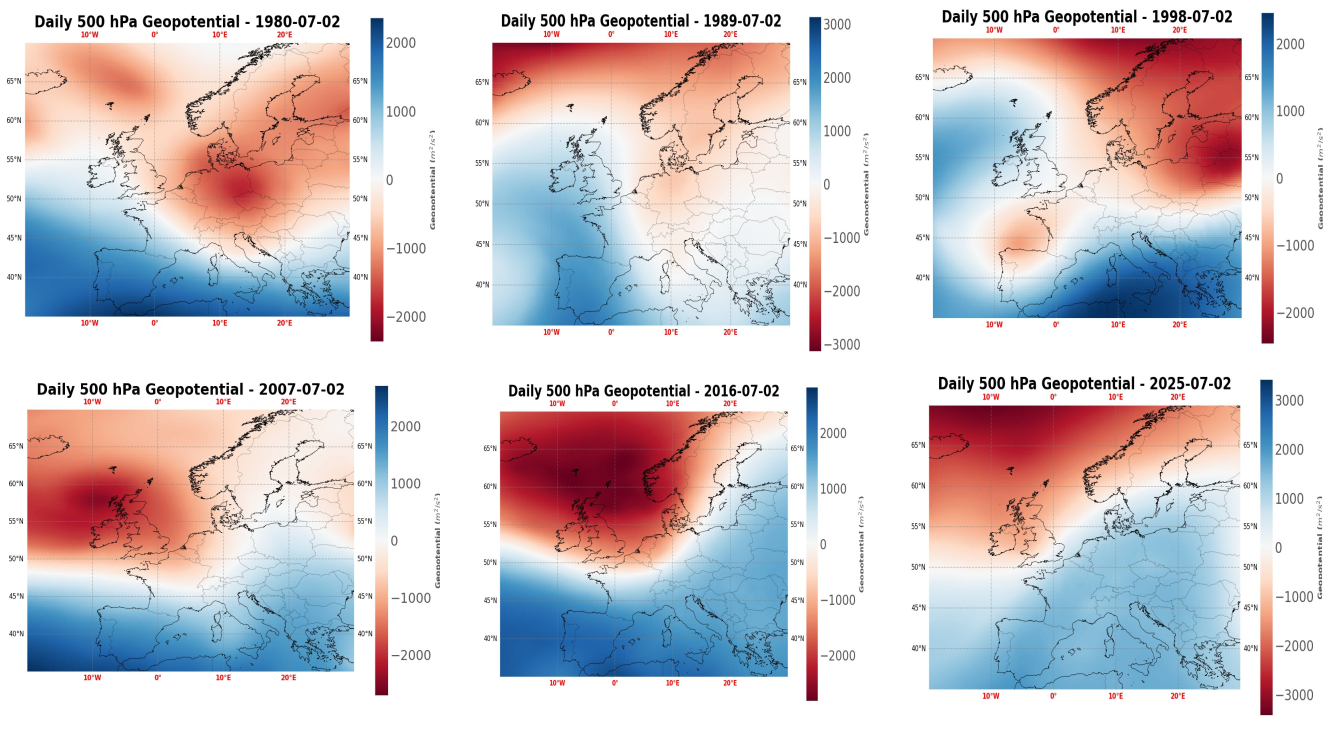
\includegraphics[height=0.55\textwidth]{figures/anys/dailys.png} \\ 
    \end{tabular}
    \label{fig:3}
\end{table}
\end{frame}

\begin{frame}[allowframebreaks]{\textbf{Mean and std for the whole dataset}}
\begin{table}
    \centering
    \begin{tabular}{cc}
        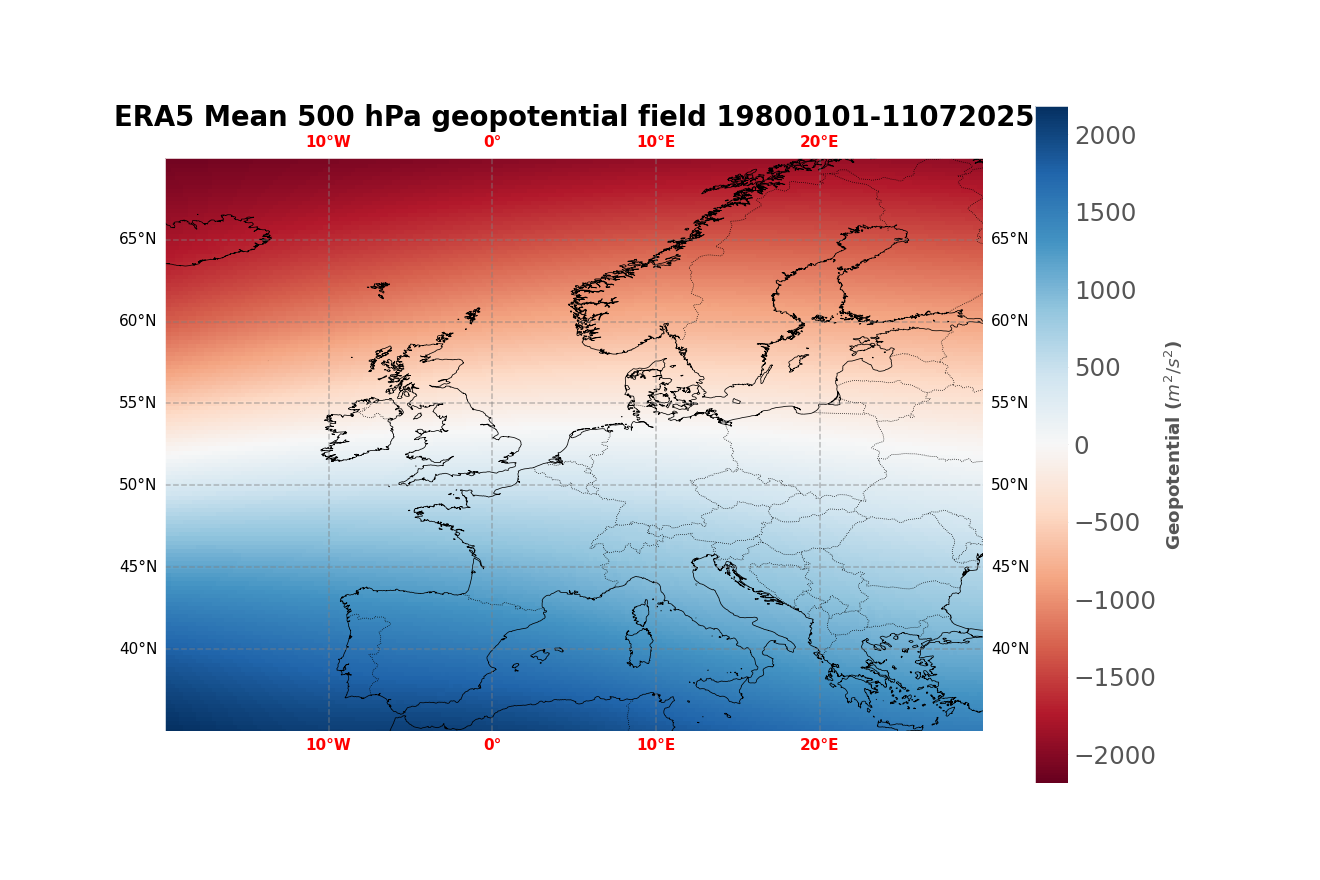
\includegraphics[height=0.4\textwidth]{/figures/danl/mean_wholeZ.png} \\ 
        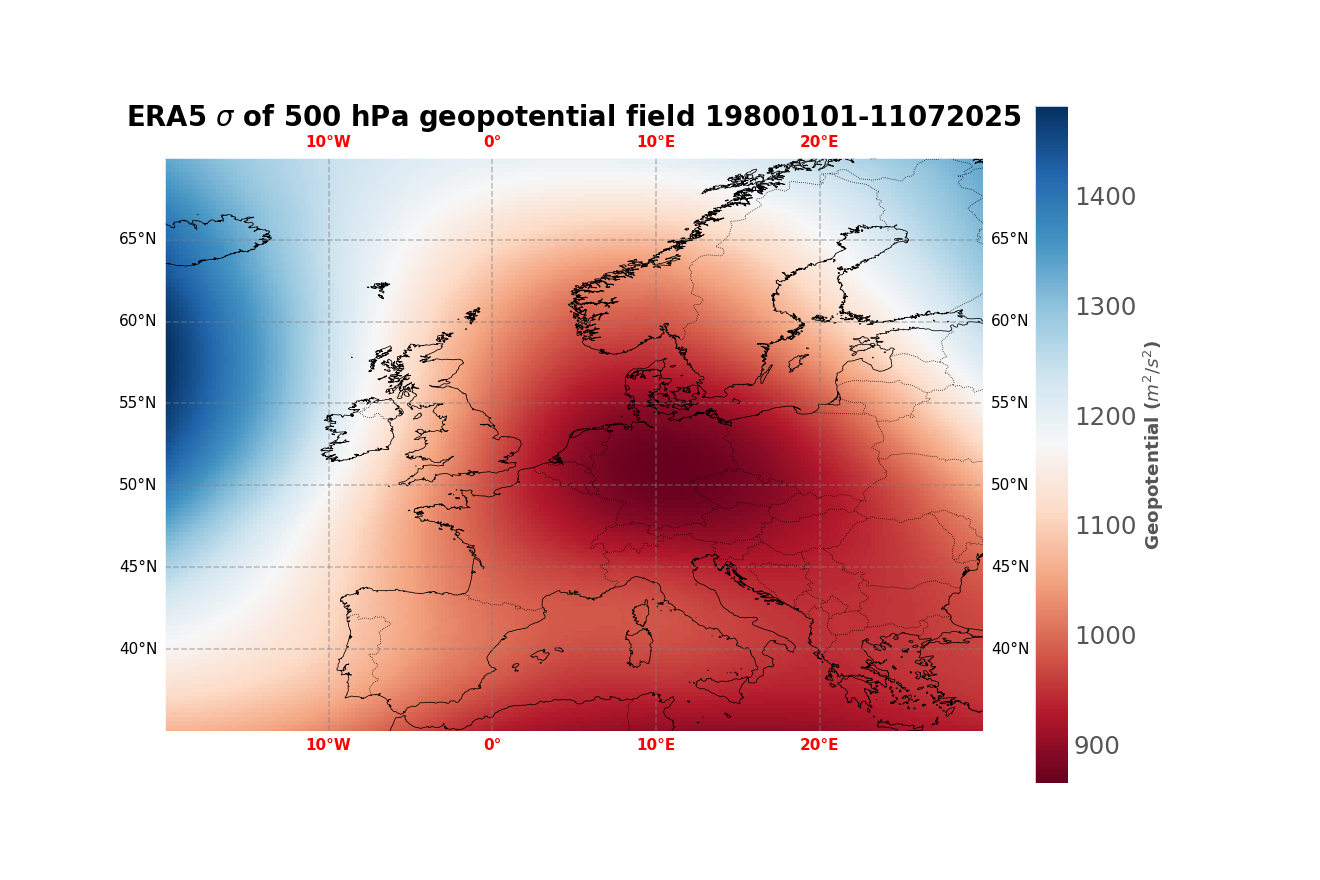
\includegraphics[height=0.4\textwidth]{/figures/danl/stddev_wholeZ.png} \\ 
    \end{tabular}
    \label{fig:4}
\end{table}
\end{frame}

\begin{frame}[allowframebreaks]{\textbf{Analysis by means of analog method}}
\begin{table}
    \centering
    \begin{tabular}{cc}
        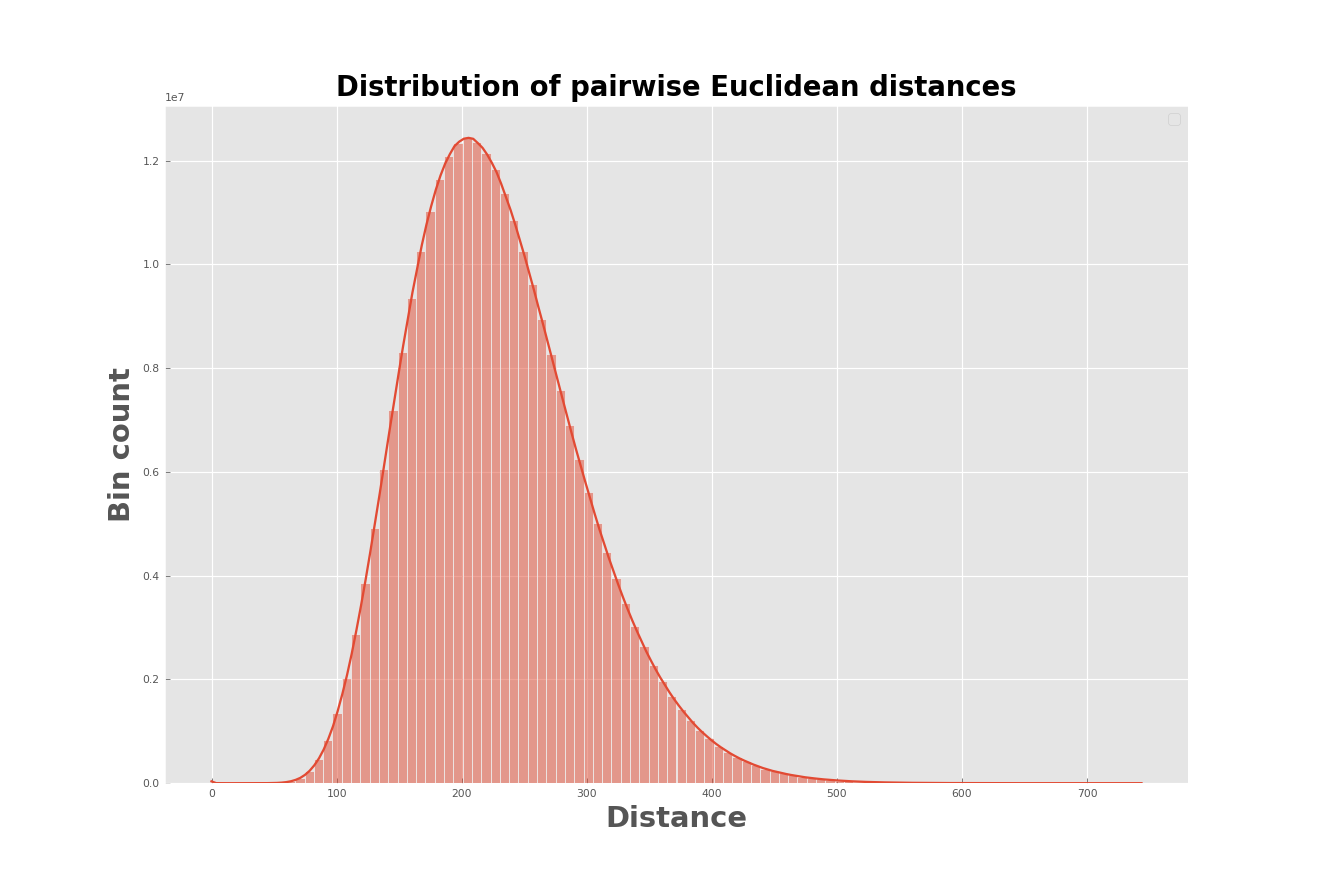
\includegraphics[ width=0.4\linewidth]{/figures/anys/euclid1.png} \\
        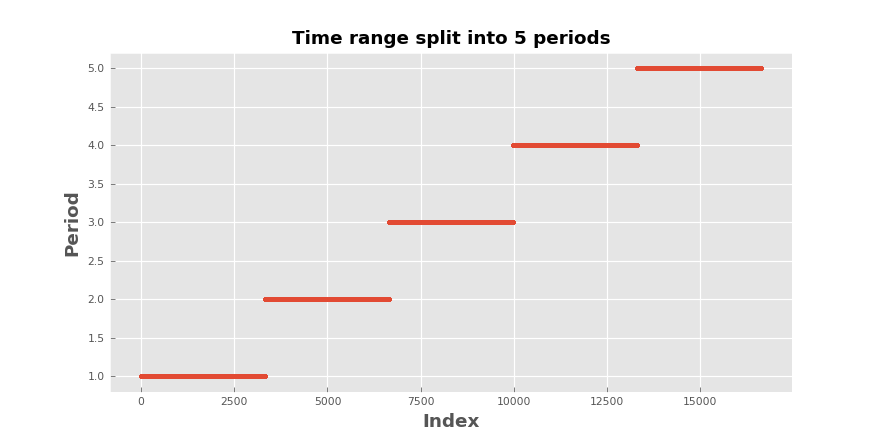
\includegraphics[height=0.20\linewidth]{/figures/anys/periods.png} 
    \end{tabular}
    \label{fig:5}
    \caption{$d_{ij}= \sqrt{\sum_k (x_{ik} -x_{jk})^2)}$, $x_{ik}$ is the generic field value at grid point k on day i while $d_{ij}$ measures \colorbox{orange}{how different two daily fields} are in physical space.}
\end{table}
\end{frame}

\begin{frame}{\textbf{Analog metrics computation}}
Below Figure \ref{fig:7}, show Euclidean distance distributions for all \textbf{six} different reference days chosen.
\begin{table}
    \centering
    \begin{tabular}{cc}
        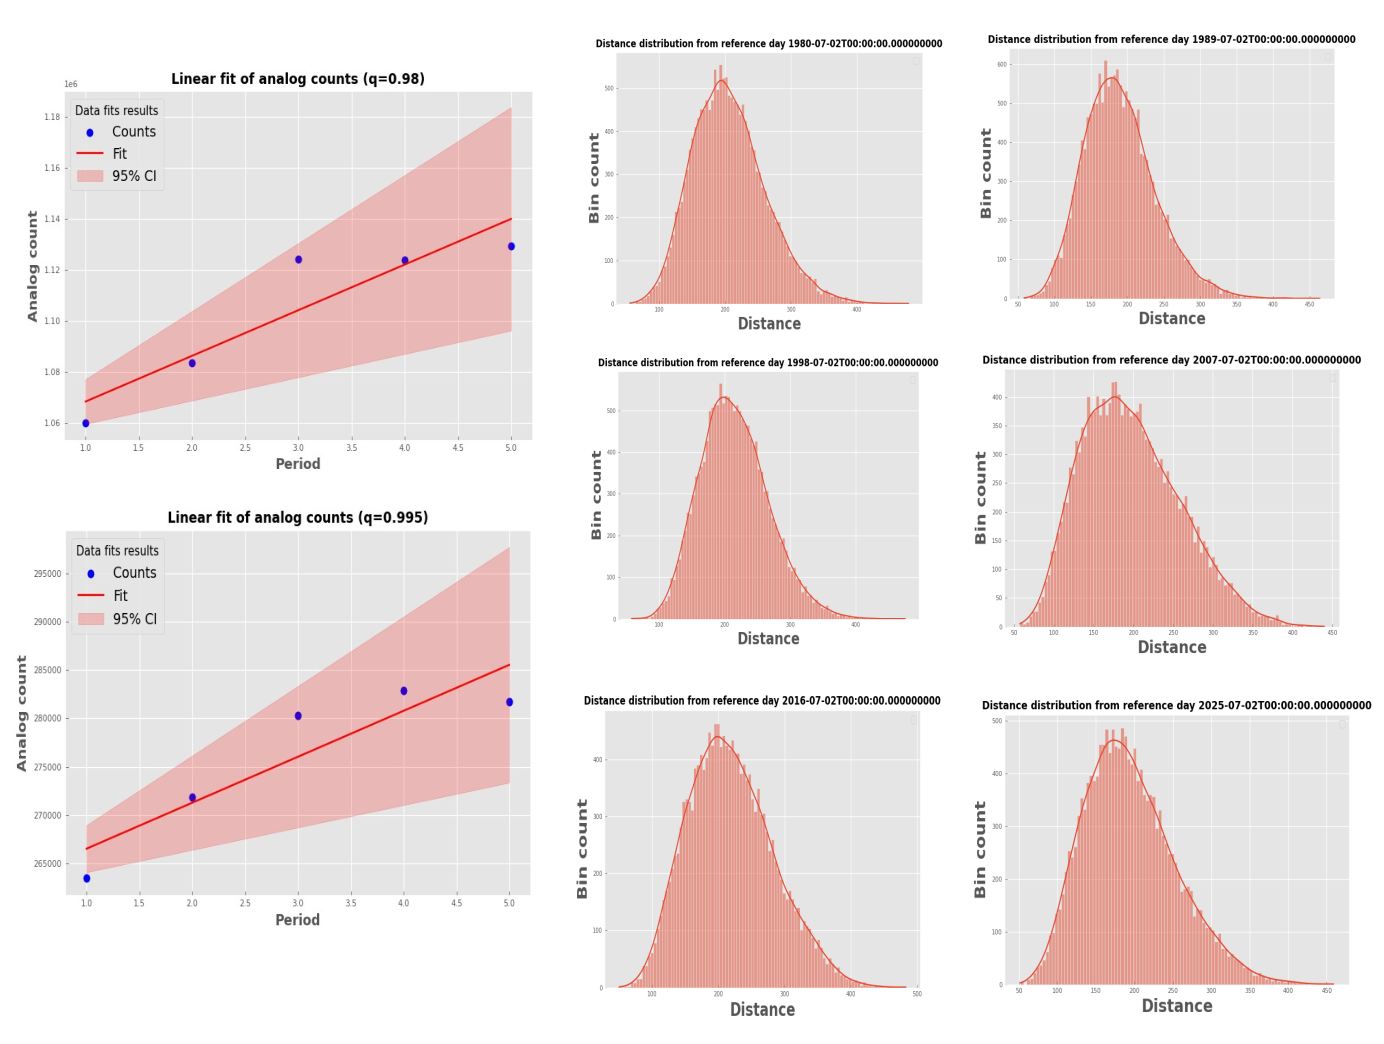
\includegraphics[width=0.75\linewidth]{figures/anys/linearfit+distr.png}
    \end{tabular}
    \label{fig:6}
  \caption{Linear fit results and confidence intervals for two different quantiles reference value. Distributions of Euclidean distances for multiple map indexes at a single reference day (16691th). The linear fit has been $N(t) = a t +b$ where N is the period of years selected following the 95\% CI.}
\end{table}
\end{frame}

\begin{frame}[allowframebreaks]{\textbf{Analysis by means of analog method}}
\Fontvi
\begin{table}
    \centering
    \begin{tabular}{cc}
        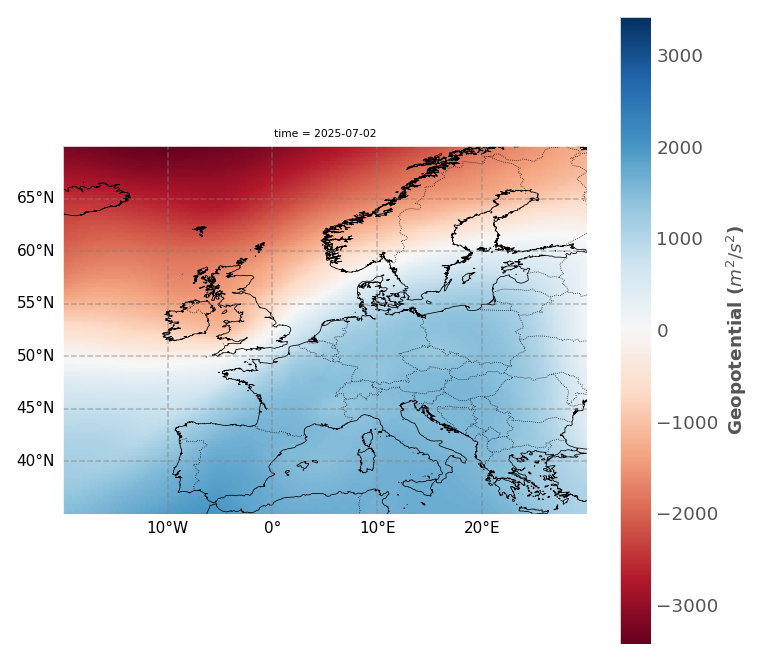
\includegraphics[ width=0.37\linewidth]{/figures/anys/reference_map_166191.png}  
        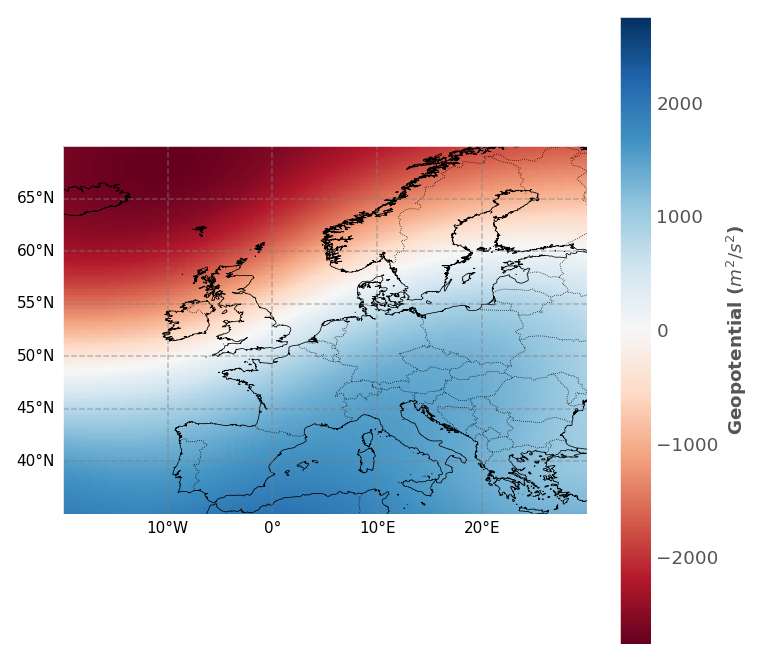
\includegraphics[ width=0.40\linewidth]{/figures/anys/mean_analogs_166191.png} \\
         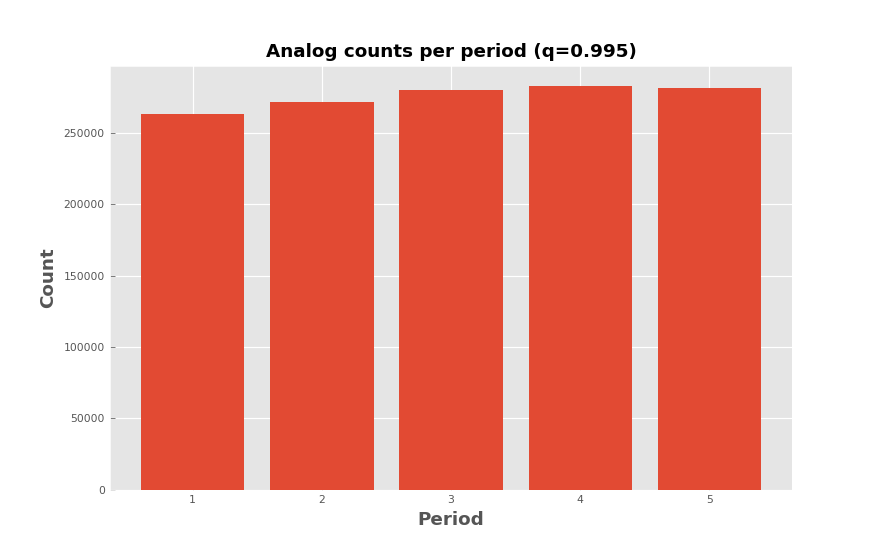
\includegraphics[width=0.31\linewidth]{figures/anys/ancountsper1_0.98_0.99_0.995_16619.png}
        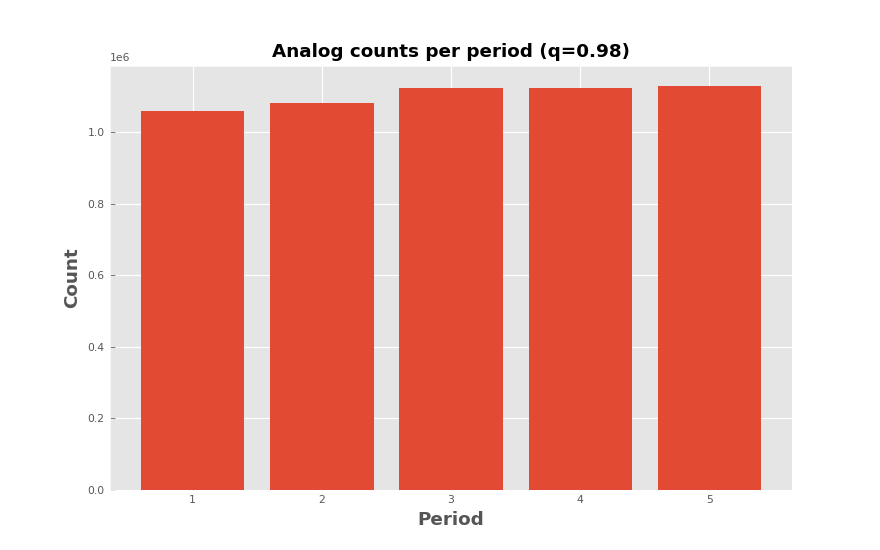
\includegraphics[width=0.31\linewidth]{figures/anys/analogcounts1_0.981.png}
    \end{tabular}
        \caption{Top images represent the analog reference map for the 16619th day and the analogs mean computed over the whole time index respectively. Bottom ones show the analogs counts for different quantiles values, the difference is not very remarkable. }
    \label{fig:7}
\end{table}
\end{frame}

\begin{frame}[allowframebreaks]{\textbf{TI1 index throughout the recurrent days}}
\begin{table}
    \centering
    \begin{tabular}{cc}
        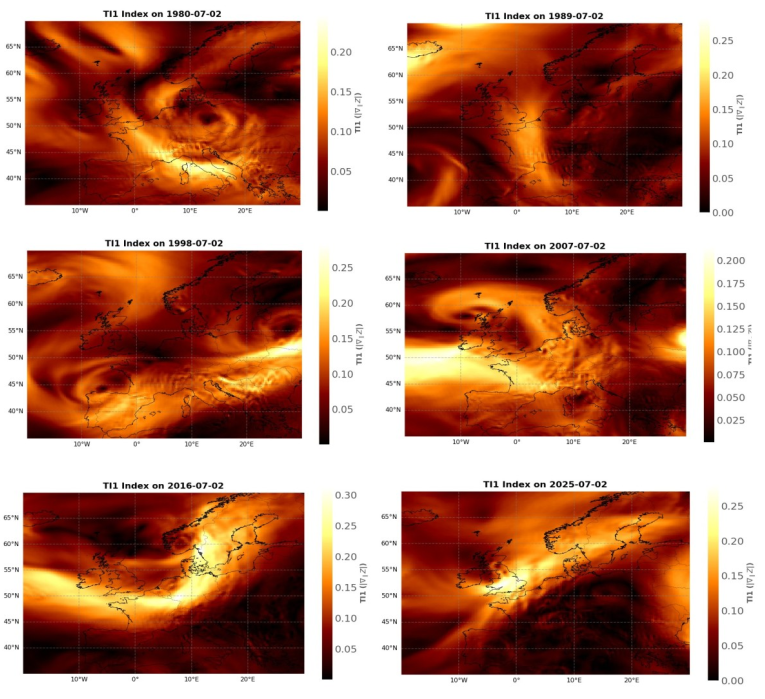
\includegraphics[height=0.56\textwidth]{figures/anys/tindexs.png} \\ 
    \end{tabular}
    \label{fig:9}
    \Fontvs
    \caption{$TI1= |\nabla z| = \sqrt{ \left(\frac{\partial z}{\partial x}\right)^2-\left(\frac{\partial z}{\partial y}\right)^2}$, \textbf{dimensionless proxy} of thermal wind strength at 500 hPa height.}
\end{table}
\end{frame}

\begin{frame}[allowframebreaks]{\textbf{Final conclusions}}
\begin{enumerate}
\item \textbf{The Euclid. distances figure} showed how similar or dissimilar daily atmospheric circulation patterns are to each other. Being it a left-skewed one, many days are similar to one another $ \longrightarrow$ common patterns.
\item How “tight” the computed \textbf{analogs} are in the feature space is found by the magnitude of distances. Namely the kernel density estimate computed with seaborn utilities.
\item If most distances are \textbf{low} $ \longrightarrow$ high pattern similarity, possibly dominated by a few regimes.
\item If distances vary \textbf{widely} $ \longrightarrow$ strong variability, with many rare patterns.
\Fontvi
\item \textbf{q=0.98}, the analogs will lie in the left tail of this distribution, namely the most similar maps. The linear fit and CI computed indicated a \colorbox{orange}{\textbf{consistent trend}}. Further investigation on larger and more broad datasets is needed (namely the other indexes reported before).
\item \textbf{TI1 remarks}, its higher values match stronger horizontal gradients $ \longrightarrow$ stronger baroclinicity $\propto \frac{1}{\rho^{2}}\vec{\nabla}\rho\times\vec{\nabla}p$ mainly a raw indicator of CAT events occurrence.
\Fontvs
\begin{table}[ht]
    \centering
    \begin{tabular}{|c|c|c|c|}
        \hline
        \textbf{Quantile ($q$)} & \textbf{Slope} & \textbf{95\% Confidence Interval} & \textbf{Ref. day} \\
        \hline
        0.98  & 17,903.600 & (9,140.823, 26,666.377) & 16619 \\
        \hline
        0.99  & 8,792.900  & (4,424.833, 13,160.967) & 16619 \\
        \hline
        0.995 & 4,756.900  & (2,318.860, 7,194.940)  & 16619 \\
        \hline
    \end{tabular}
    \caption{Slope coefficients and 95\% confidence intervals for different quantile thresholds ($q$) corresponding to reference day 16619.}
    \label{tab:slope_CI}
\end{table}
\end{enumerate}
\end{frame}

\begin{frame}[allowframebreaks]{\textbf{Bibliography}}
 
\Fonttab
\scriptsize
\bibliographystyle{apalike}
\bibliography{bib/references}
\end{frame}

\end{document}
